% sections/intro.tex: Section 1. Numbers: results/rho_within_readings.csv (within_reading.R), results/experiments_rho_summary.csv
% (experiments_ledger.R), results/panel_windows_auto.csv, results/identification_within_person.csv, identification_deficiency_powered.csv,
% equity_margin.csv, identification_person_place_v2.csv, scf_beliefs_by_group.csv.
\section{Introduction}\label{sec:intro}

A borrower deciding whether to default on a loan makes an intertemporal choice: forgo the payment due now and consume more today, at the cost of penalties that reduce future utility. In an endogenous-default model with concave, time-separable utility, the response of default to a payment due $s$ months ahead is the product of a scale common to every date and a weight specific to the date: the discount function $D(s)$, the probability $Q(s)$ of still facing the payment, and the marginal utility of a dollar at $s$ relative to a dollar at today's default threshold. The ratio of the responses to two payment paths in the same population cancels the scale, and with survival measured it identifies $D$ without consumption data, income paths, or a functional form for utility (Section \ref{sec:suffstats}; Appendix \ref{appendix:multiperiod} states the model in full). It replaces ``marginal willingness to save,'' the identifying variation of asset markets, with ``marginal willingness to avoid default,'' and makes time-preference measurement possible for the households who hold debt and no financial assets. Applied within borrower to a credit-bureau panel of auto loans, the identity gives the paper's estimate: an annual discount rate of $0.11$, with a 95 percent set from $0.09$ to $0.13$, the loan-weighted mean across credit-score deciles of the rates that borrowers reveal when two of their own loans are compared. The decile estimates run from $0.01$ to $0.22$, and only the sets of the two highest deciles, where defaults are rare, include zero. Applied to the published experiments that move payments at known dates by rule, the same identity is a check rather than a benchmark: the pair of arms in \citet{dobbie_targeted_2020} that moves payments at two future dates in one population fits best at a rate of zero over four years and accepts every rate from zero to $1.2$ at the five percent level once its five-year outcome window is aggregated over the decision months it contains. The experiment fixes the sign and the horizon of the far-payment response; the bureau's contract fixes its level, because the far payment of a five-year contract sits near the horizon at which a payment response identifies the rate most precisely, and the paper shows why no published experiment sits there. The estimate is half the median laboratory elicitation of $0.22$ per year \citep{cohen_measuring_2020} and more than five times the two percent social discount rate of federal cost-benefit analysis \citep{the_white_house_biden-harris_2023}. Figure \ref{fig:rho_headline} shows the estimate by credit score and by income.

\begin{figure}[H]
\centering
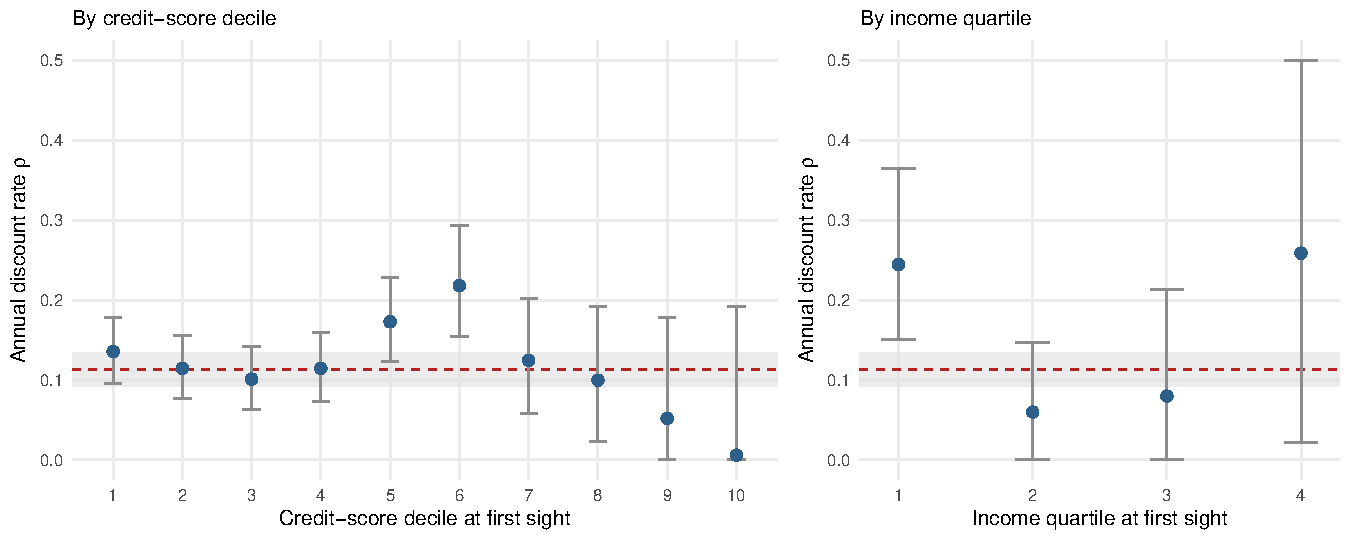
\includegraphics[width=0.9\textwidth]{figures/fig_rho_headline.pdf}
\caption{The rate. The within-borrower estimate of the annual discount rate by credit-score decile (left) and by income quartile (right), with 95 percent sets; the dashed line is the loan-weighted mean across deciles, $0.11$, and the band its 95 percent set (Section \ref{sec:rate_people}).}
\label{fig:rho_headline}
% replication: Code/local/within_reading.R, Code/exhibits/make_rho_headline_figure.R
\end{figure}

Three measured objects produce the number, and each has published counterparts, which is what a sufficient-statistics formula is for. The first is the response of default to the monthly payment: an elasticity of $0.45$ on 7 million auto loans within cells of lender, place, score and income, and $0.53$ within borrower on the 13.5 million borrowers with two or more auto loans in a ten-percent archive of credit files, 65 million loans. The second is the response of default to the contract's length at a fixed payment, which adds payments at the far end of the contract: $0.30$ within borrower at twenty-four months. The third is survival, the hazard at which a loan ends for a reason other than default, $0.19$ per year net of servicer transfers. The payment response has counterparts in every quasi-experiment that moved a mortgage or card payment by rule, and Table \ref{tab:benchmark} sets them beside the bureau's at the two margins the literature distinguishes, a payment change with the balance moving and one at a fixed balance. The far-payment response has counterparts in the two-arm experiments, to which Section \ref{sec:quasi} applies the same weights; a reader who prefers a published estimate of any input can substitute it and recompute the rate.

The credit bureau's contribution is the population and the designs. Auto loans reach the low end of the income and credit-score distributions, the households whose time preferences asset prices do not reveal and whom laboratory samples do not reach, and the panel records the score, income, lender and location of every loan. Four designs in these data identify a response without any assumption about who chooses which contract; three have their own subsections in Section \ref{sec:autodata}, and the fourth is in Appendix \ref{appendix:traits}. Within-borrower comparisons hold the person fixed and identify the payment and far-payment responses net of every stable trait; run group by group, they give the rate by score decile, income quartile and age (Section \ref{sec:rate_people}). State laws that bar lenders from pursuing the unpaid balance after repossession, and the recourse laws of mortgage states, identify the penalty channel of the term margin: where the balance cannot be pursued, a longer contract lowers early default by $0.36$ ($0.13$) less per unit of log length on small auto loans and by $3.9$ ($1.5$) less on mortgages, the cost of default rising with what is owed (Section \ref{sec:termmargin}). House-price movements across purchase cohorts within a zip code and quarter identify the walk-away response of mortgage default to negative equity, an elasticity of $-2.5$ that is stronger where the law bars recourse and convex in the shortfall (Section \ref{sec:equity}). And borrowers who move between areas identify the place's share of the geography of default, one tenth (Appendix \ref{appendix:traits}). A reader who accepts nothing else in the paper still has these.

The population step is not optional, and it rests on the designs. Simple fixed-effects regressions on every loan, benchmarked against the within-borrower estimates and the published quasi-experiments and interpreted as causal under a stated assumption, are what give heterogeneity at population scale with power (Section \ref{sec:identification}). What they show is that the heterogeneity in default across people is heterogeneity in exposure to the default margin, the density of borrowers at the threshold, and not in the rate: the payment elasticity is $0.41$ in the bottom income quartile and $0.86$ in the top, and the score-decile profile peaks near the median, while the within-borrower rate has no gradient in score or income (Section \ref{sec:heterogeneity}). The experiment that reports both of its arms by subgroup finds the same: the rate is the same above and below the median credit score and the median debt-to-income ratio (Section \ref{sec:quasi}). The one gradient in the bureau is age: borrowers aged 18 to 30 reveal a rate of $0.32$, with a set from $0.21$ to $0.48$, and every older group reveals zero.

Ahead of the exponential rate sits a premium on the payment due now. The marginal-utility ratio $\lambda$ of a repayer at a later date to the marginal defaulter today multiplies every future weight, and Section \ref{sec:results} shows that the present-bias parameter of \citet{laibson_golden_1997} and this ratio enter every default response as a product: in this class of models no comparison of a payment due now with payments due later separates them, and in that sense they are the same object. The paper measures the product from the one published comparison that holds the date fixed and varies the currency, the payment-relief and seizable-equity responses in \citet{indarte_moral_2023}, at $\lambda = 0.2$ as the level of a profile that declines with the horizon as the distress state mean-reverts, and states the assumption under which that ratio is the model's $\lambda$. The main text reports one exponential rate under time-consistent preferences with the premium as one measured number; the rate beyond the first payment is insensitive to it, and Appendix \ref{appendix:nonclassical} states what would identify its parts.

The estimates hold beliefs at their measured values. Survival enters every weight, so a borrower who expects to leave her loan sooner than the measured hazard would reveal a higher rate than she has; and a borrower who expects her income to recover weighs a later dollar less than the objective persistence of distress implies, which enters the premium. Neither belief is in the bureau's data. The 2022 Survey of Consumer Finances asks households what they expect of their own income, and Appendix \ref{appendix:beliefs} sizes both channels: constrained households expect a recovery of $0.11$ log points against $0.02$ for the unconstrained, the default-side correction to the rate is bounded by the group's default hazard, at most $0.06$ in the lowest score decile, and the expected recovery accounts for a first-year discount of 16 to 28 percent that sits inside the measured premium and is neither liquidity nor impatience.

Why must we look beyond asset prices? The Euler equation prices risk-free bonds using the discount factor of the \emph{marginal investor}, who is presumably wealthy and patient. The time preferences of the remaining households, the constrained, the hand-to-mouth, the borrowers, are not identified by these prices. Laboratory experiments offer an alternative, but the relevance of lab-elicited discount rates to real-world financial decisions is unclear, in part because behavior under small stakes may differ substantially from behavior under large stakes \citep{coller_eliciting_1999, harrison_estimating_2002, rabin_risk_2000}. The approach developed here uses real-stakes decisions at economically meaningful time horizons, observed at population scale.

The estimates have implications for credit policy and for public finance. For credit policy, the premium says that a dollar of relief on the payment due now prevents more default than a dollar of relief on a payment due later, by the factor $1/\lambda_s$, from $1.1$ for a payment due next month to about $3$ for one due five years out, and the two-arm experiments say the same only once their arms are classified by the sign of every month's payment change: a rescheduling that lowers payments now and adds them later is not relief, and its value to a borrower depends on the weights the formula assigns to the dates it moves payments between. For public finance, the estimate of $0.11$ is more than five times the two percent social discount rate the federal government applies, and \citet{hendren_unified_2020} show that the ranking of early-childhood against adult programs turns on rates in this range; for the households whose rate this is, the finding raises the value of programs with near-term payoffs relative to programs whose returns arrive decades later.

The paper proceeds as follows. Section \ref{sec:literature} states what the related literatures find and what this paper adds. Section \ref{sec:data} describes the panel. Section \ref{sec:suffstats} sets out the model, the sufficient-statistic results and their three provisos, the mapping from responses to a rate, and the published experiments. Section \ref{sec:autodata} applies the mapping to the credit-bureau panel, one design per subsection; Section \ref{sec:heterogeneity} reports exposure at population scale; Section \ref{sec:comparison} compares the estimates with prior work, Section \ref{sec:discussion} discusses what the rate and the premium capture, and Section \ref{sec:conclusion} concludes. The appendices prove the results, size the beliefs the estimates condition on, relax the classical preference restrictions, report every design in full, record the designs that do not identify the rate, and document the data and the replication of every exhibit.
